\section*{\begin{center}{Appendix D}\end{center}}
\addcontentsline{toc}{section}{Appendix D}
%$\\[0.5cm]$

\section*{Additional experiment results}

Included in this appendix are figures created from the experiment results of the experiments on the DG-weighting, and the experiments on the neuronal turnover rate, $\tau$, as referred to in chapter \ref{chpt:experiments}. Additionally, the figures of training on the second subset in the low-level demonstration are included.

% \subsection*{Further figures from experiment 4.2, DG-weighting}

\begin{figure}[h!]
    \centering
    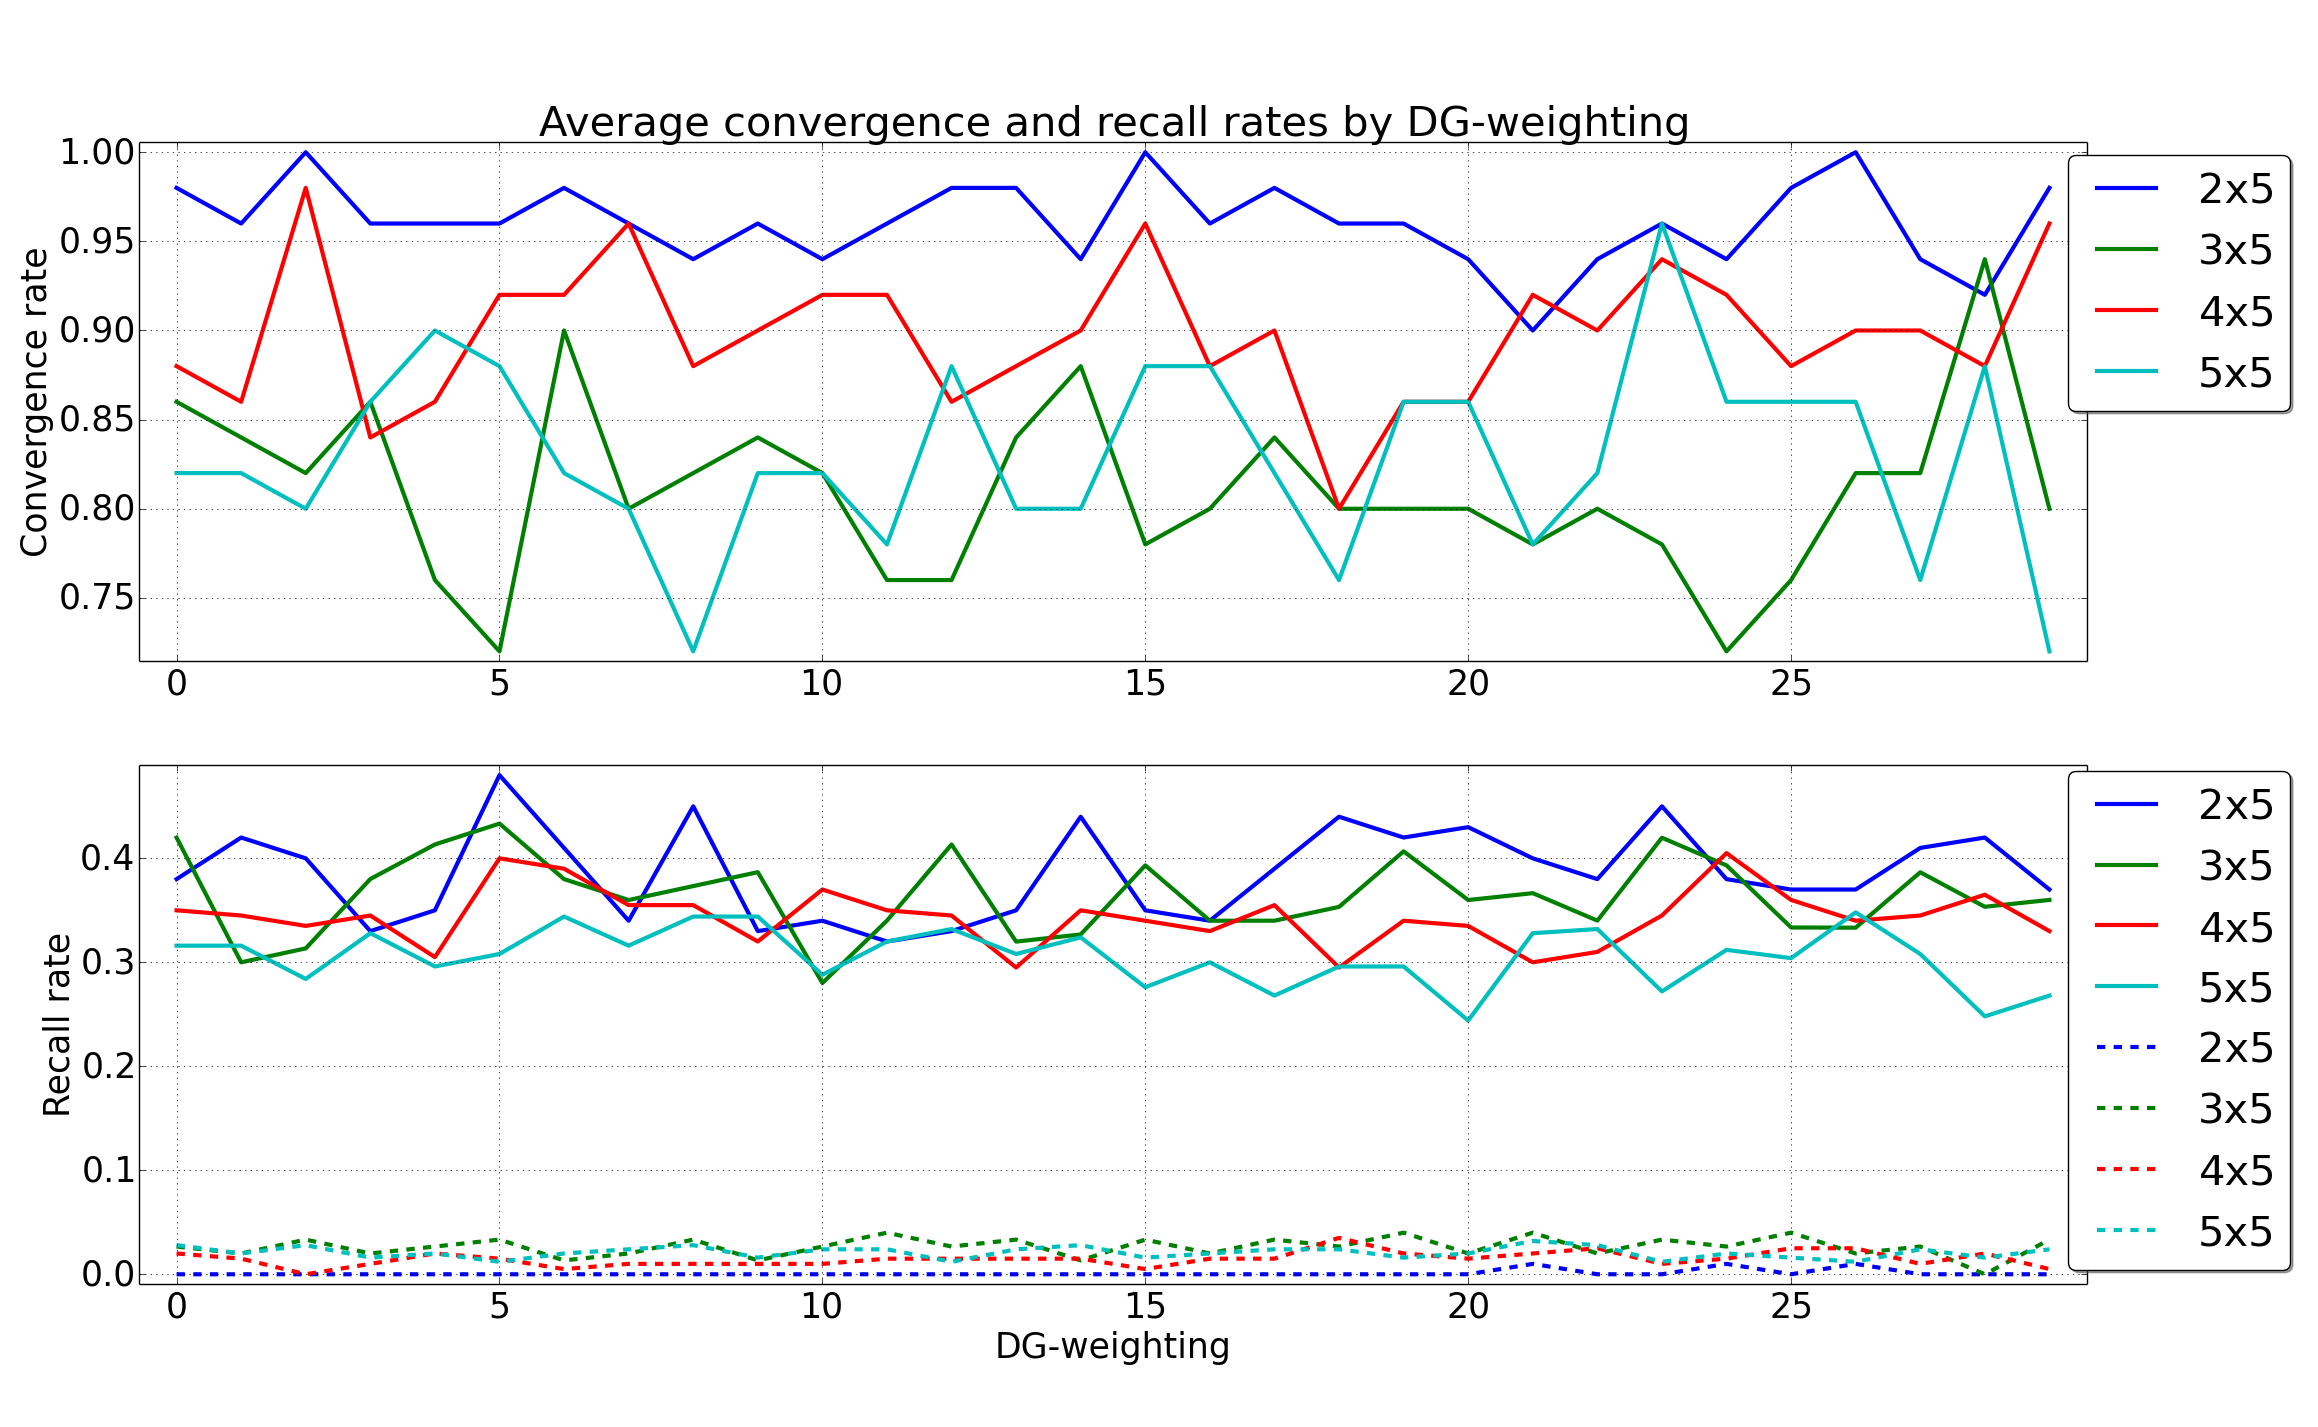
\includegraphics[width=13cm]{fig/DGWs/sync_tm1_04}
    \caption{Showing the results attained for \textbf{convergence and recall rates by the DG-weighting} when using \textbf{synchronous} CA3-layer updating and neuronal turnover for \textbf{every training iteration}, $\tau=0.04$.}
    \label{fig:sync_tm1_04}
\end{figure}

\begin{figure}
    \centering
    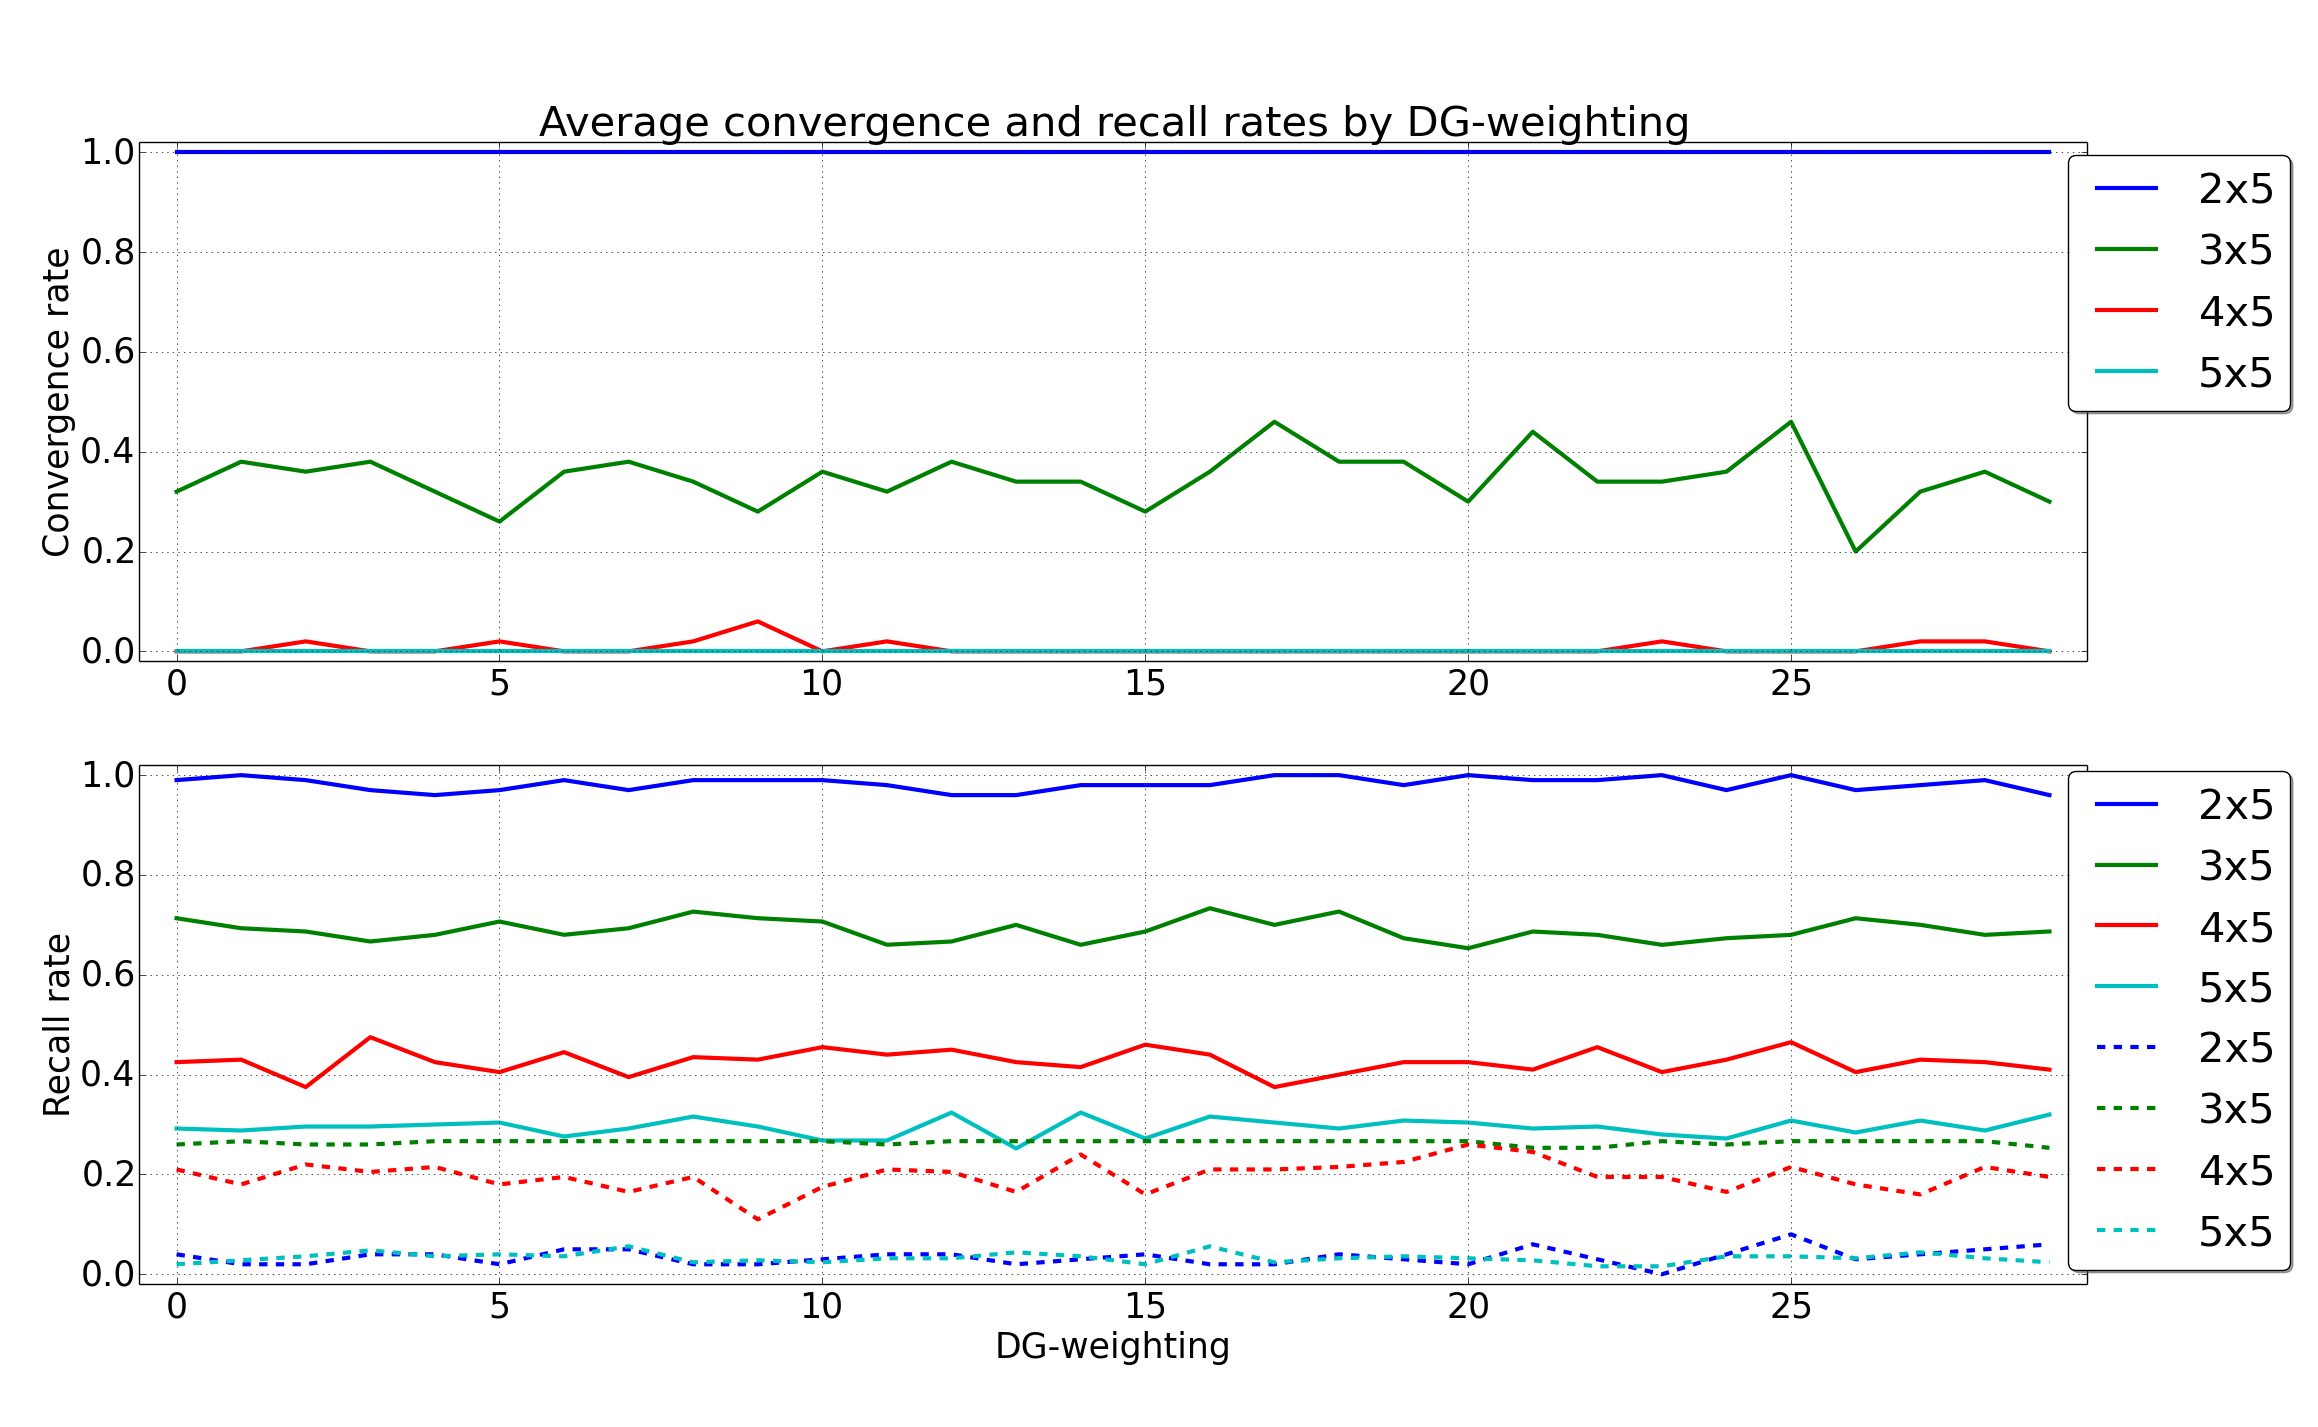
\includegraphics[width=13cm]{fig/DGWs/async_tm1_04}
    \caption{Showing the results attained for \textbf{convergence and recall rates by the DG-weighting} when using \textbf{asynchronous} CA3-layer updating and neuronal turnover for \textbf{every training iteration}, $\tau=0.04$.}
    \label{fig:async_tm1_04}
\end{figure}

% \subsection*{Further experiment 4.3 figures: Neuronal Turnover Rates}

\begin{figure}
    \centering
    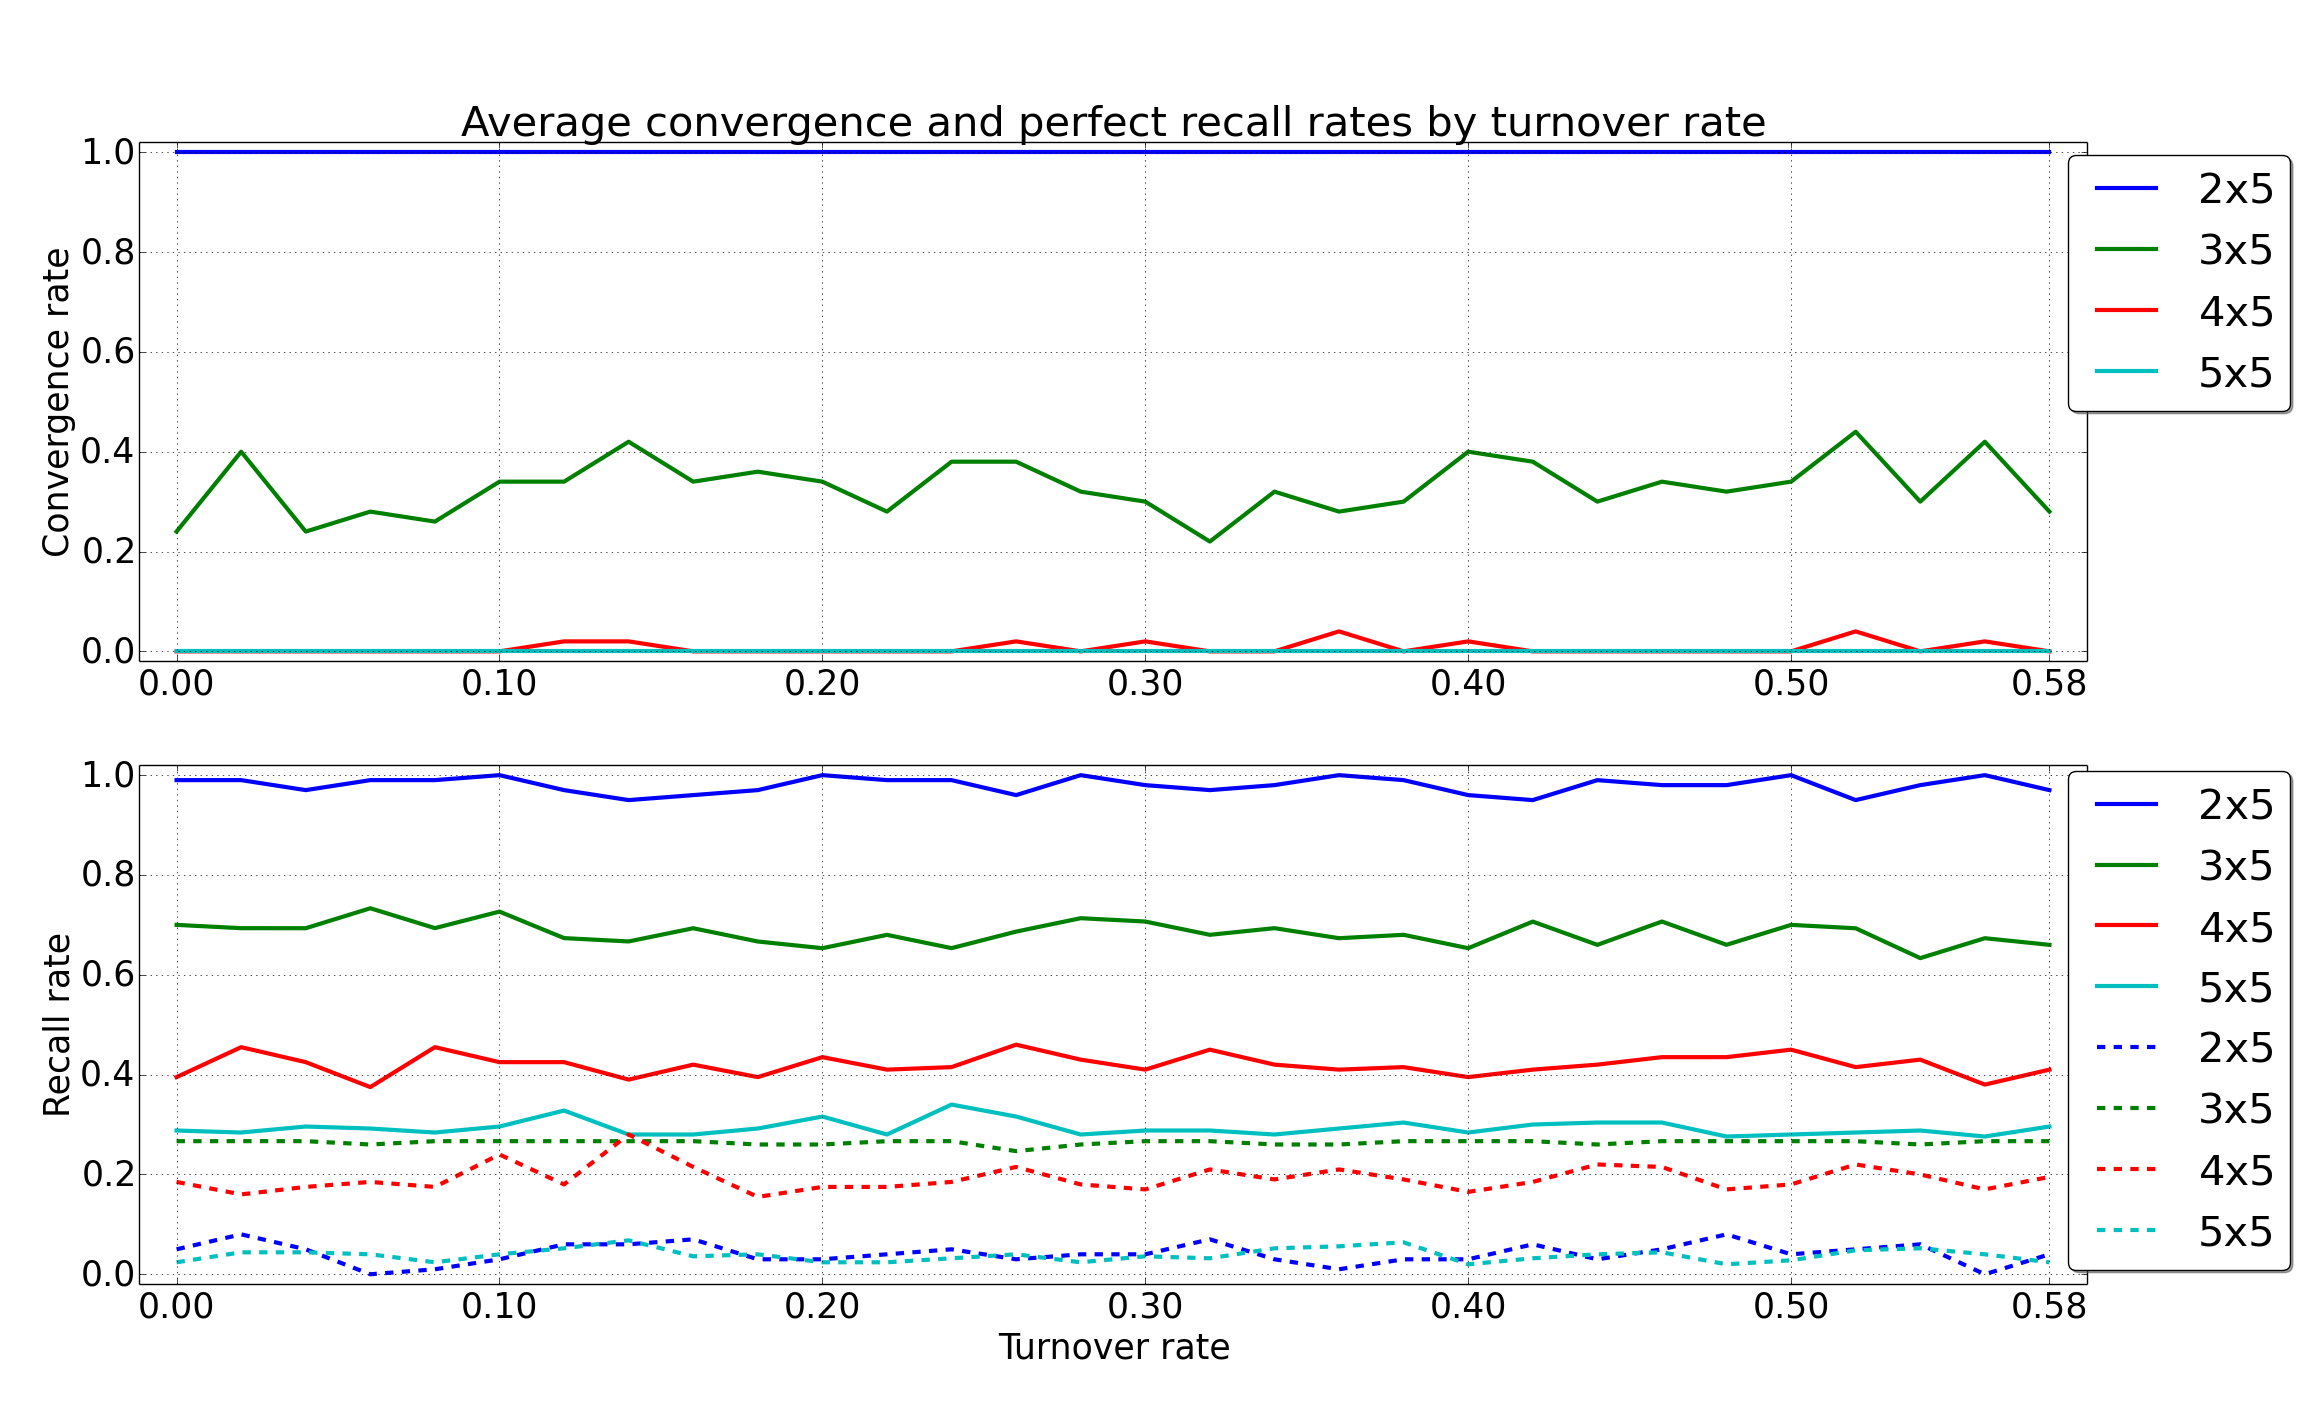
\includegraphics[width=13cm]{fig/turnover_rates/async_tm0_dgw25}
    \caption{Displaying the average \textbf{convergence- and perfect and spurious recall rates by the neuronal turnover rate} for \textbf{asynchronous} CA3-updating, using a \textbf{DG-weighting of 1}, and turnover between \textbf{every learnt training subset}, with $\tau=0.50$.}
    \label{fig:async_tm0_dgw25}
\end{figure}

\begin{figure}
    \centering
    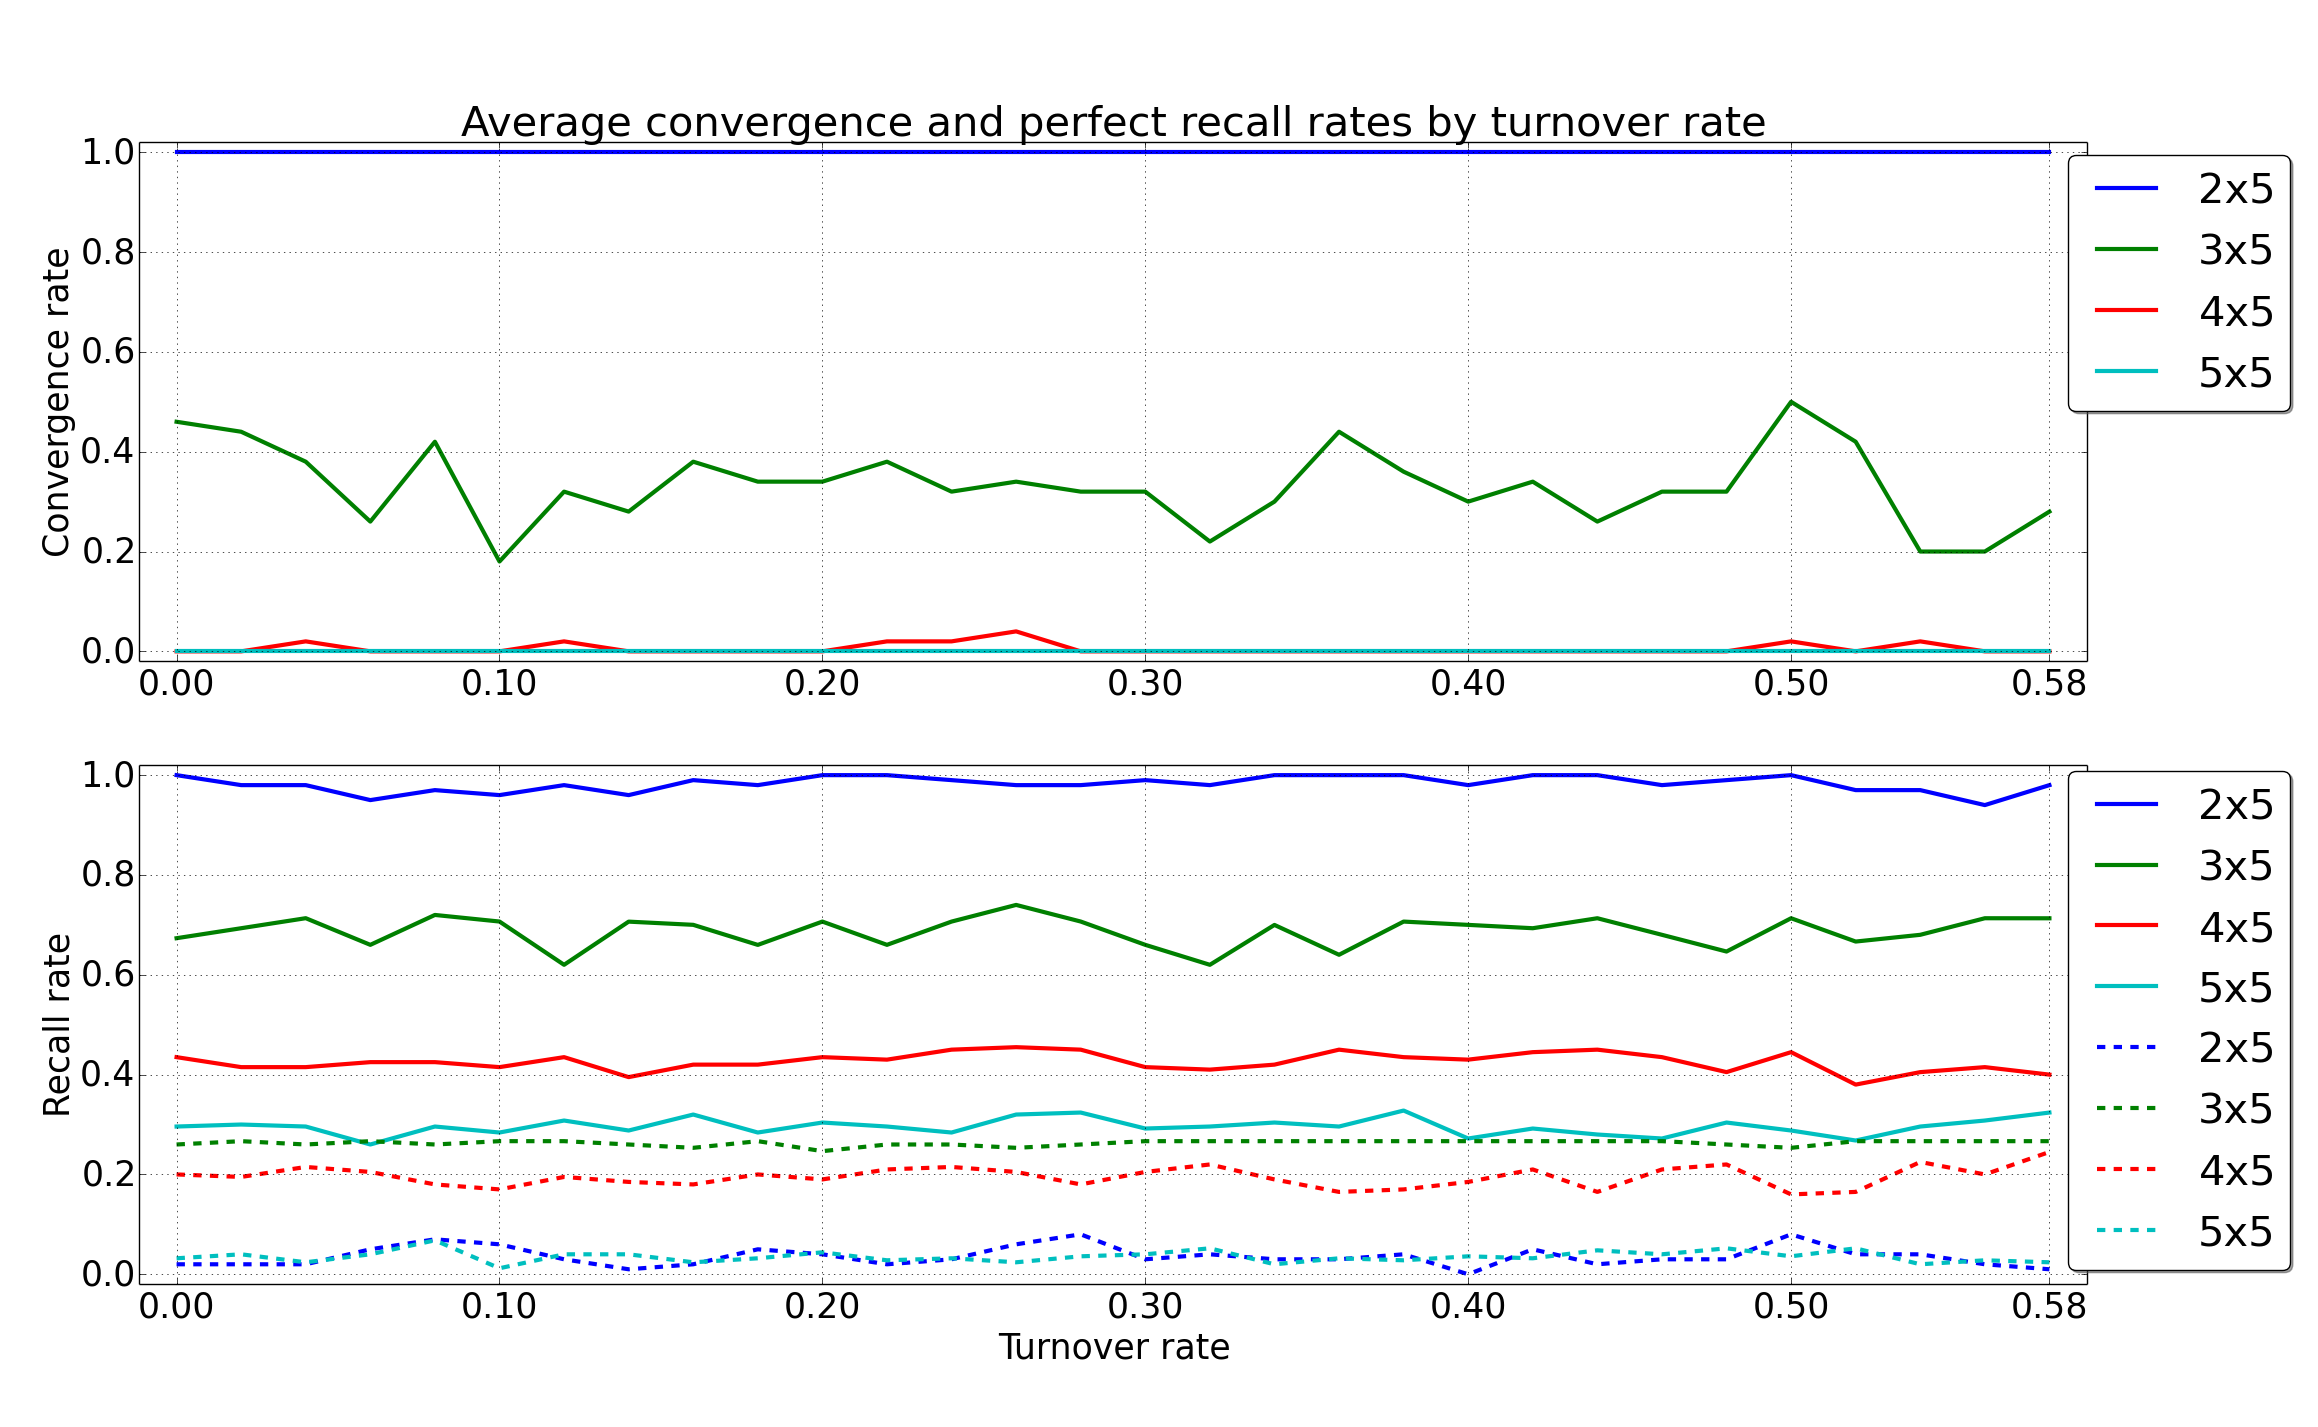
\includegraphics[width=13cm]{fig/turnover_rates/async_tm1_dgw1}
    \caption{Displaying the average \textbf{convergence- and perfect and spurious recall rates by the neuronal turnover rate} for \textbf{asynchronous} CA3-updating, using a \textbf{DG-weighting of 1}, and turnover for \textbf{every training iteration}, $\tau=0.04$.}
    \label{fig:async_tm1_dgw1}
\end{figure}

% Low-level demo.:

\begin{figure}
    \centering
    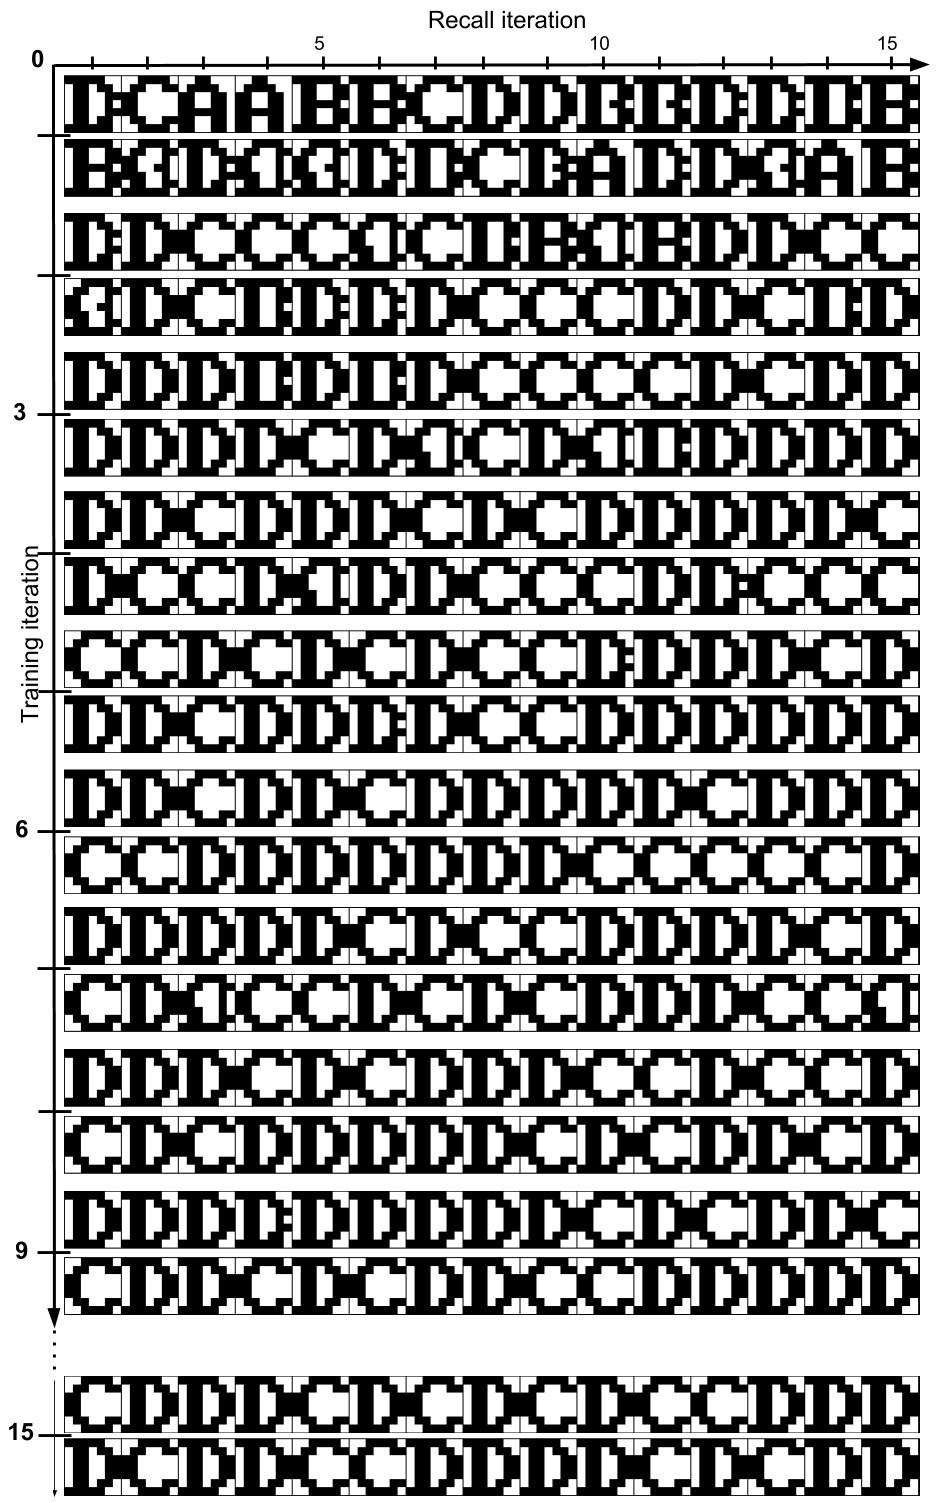
\includegraphics[width=10cm]{fig/CD-pattern-associations-async-tm0-dgw1-tau050}
    \caption{Displaying the \textbf{recall for the two patterns inputs of the training set for each training iteration}. Output is displayed in two rows per training iteration, corresponding to the training inputs 'C' and 'D', consecutively. Note that the origin is in the upper left corner. Furthermore, the model setup which is used is: \textbf{Asynchronous} CA3-layer updating, neuronal turnover between \textbf{every learnt subset}, i.e. not throughout the results displayed in this graph, a \textbf{DG-weighting of 1}, and a turnover rate $\tau=0.50$.}
    \label{fig:low-level-demo-async-tm0-dgw1}
\end{figure}

\begin{figure}
    \centering
    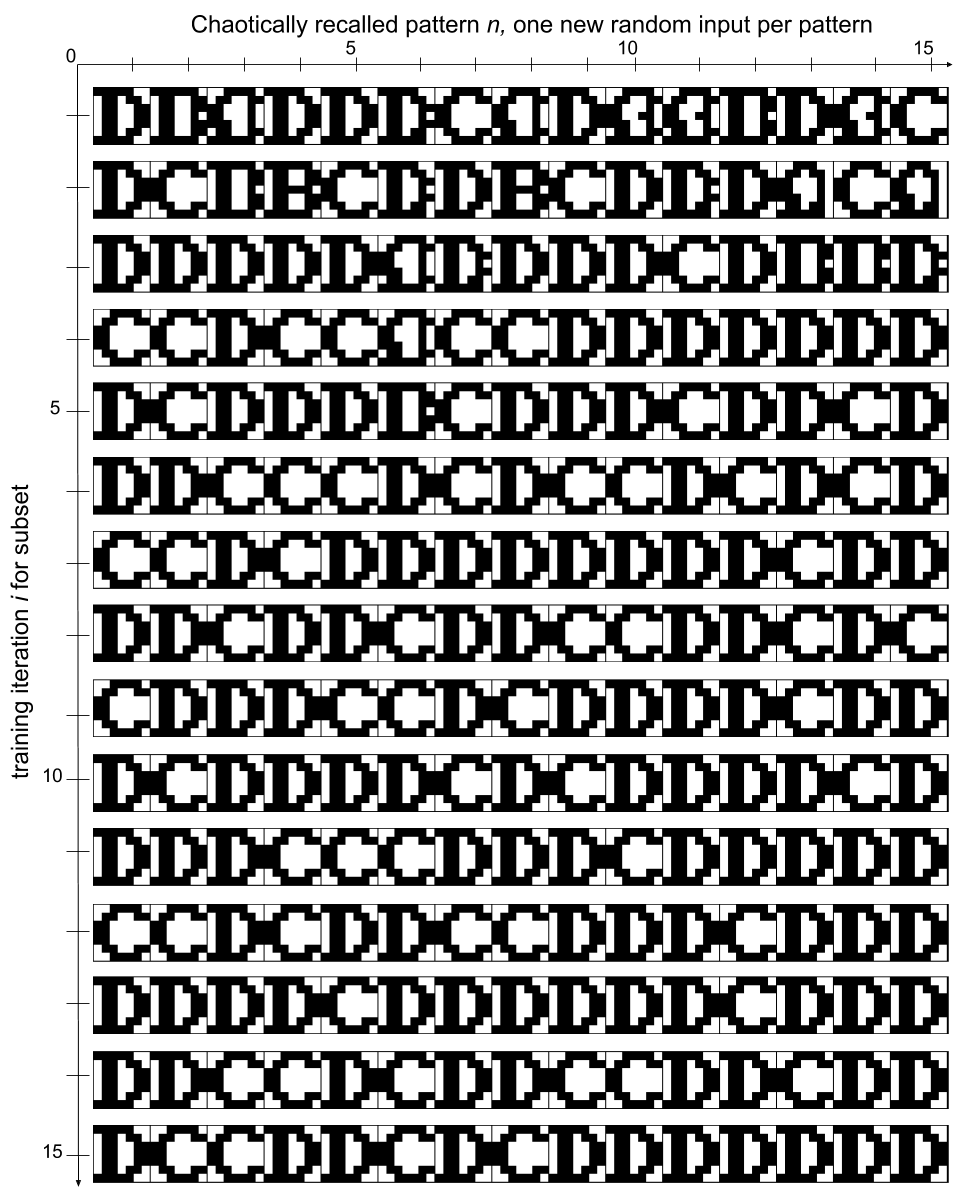
\includegraphics[width=12cm]{fig/CD-chaotic-recall-async-tm0-dgw1-tau050}
    \caption{Displaying the chaotically extracted outputs by training iteration. That is, one random input is provided to the network after each training iteration on the subset {C, D}, for which the output is displayed after every recall iteration. The model scheme corresponds to that above in figure \ref{fig:low-level-demo-async-tm0-dgw1}.}
\end{figure}

\cleardoublepage